\begin{figure}[h]
	\centering
	\setlength{\resLen}{1.5in}
	\addtolength{\tabcolsep}{-4pt}
	\begin{tabular}{ll@{\hspace{8\tabcolsep}}ll}
		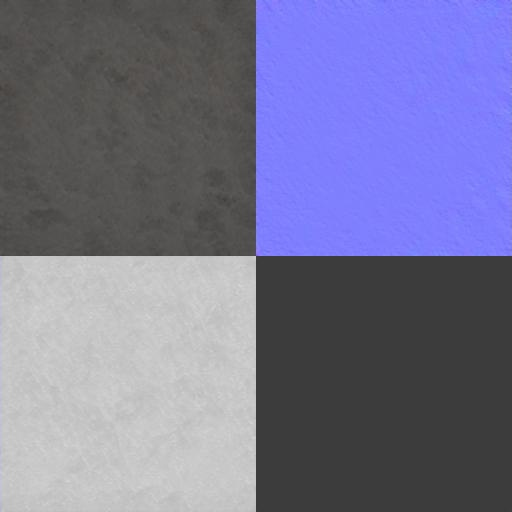
\includegraphics[width=\resLen]{svbrdf/validation/init/latent_avg_256_2x2.jpg} &
		
\includegraphics[width=\resLen]{svbrdf/validation/init/latent_avg_256_render.jpg} &
		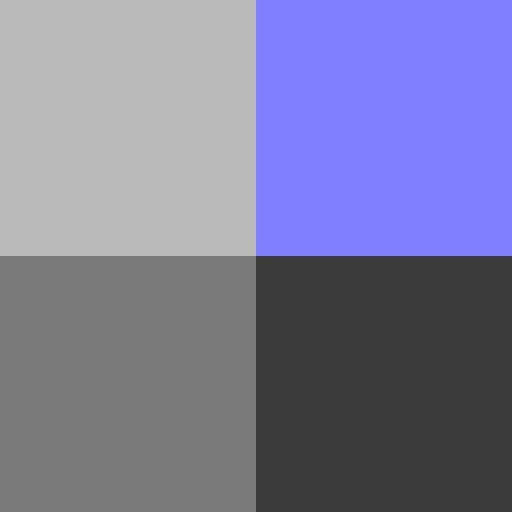
\includegraphics[width=\resLen]{svbrdf/validation/init/latent_const_256_2x2.jpg} &
		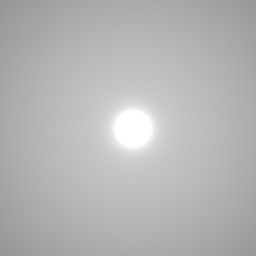
\includegraphics[width=\resLen]{svbrdf/validation/init/latent_const_256_render.jpg}
		\\
		\multicolumn{2}{c}{(a) Mean $\bmw$ initialization} & 
		\multicolumn{2}{c}{(b) Low roughness initialization} \\
	\end{tabular}
	\caption[Visualization of our constant initializations]{\label{fig:svbrdf:init}
		\textbf{Visualization of our constant initializations.} We initialize our optimization with the two materials shown here and pick the result with the lowest final loss. (This applies in cases where we do not use the result from Deschaintre et al. as initialization, as detailed in the results section and supplementary materials.) Left: Material maps generated from the mean latent vector $\bmw$. Right: An additional low roughness, specular initialization.
	}
\end{figure}